% This is the first draft of MMU Faculty of Engineering Cryptography and Security systems assignment
% for 18/19 Trimester 2
% Chia Jason 1161300548
% Hor Sui Lyn 1161300122
%



\documentclass[runningheads]{llncs}\usepackage[]{graphicx}\usepackage[]{color}
% maxwidth is the original width if it is less than linewidth
% otherwise use linewidth (to make sure the graphics do not exceed the margin)
\makeatletter
\def\maxwidth{ %
  \ifdim\Gin@nat@width>\linewidth
    \linewidth
  \else
    \Gin@nat@width
  \fi
}
\makeatother

\definecolor{fgcolor}{rgb}{0.345, 0.345, 0.345}
\newcommand{\hlnum}[1]{\textcolor[rgb]{0.686,0.059,0.569}{#1}}%
\newcommand{\hlstr}[1]{\textcolor[rgb]{0.192,0.494,0.8}{#1}}%
\newcommand{\hlcom}[1]{\textcolor[rgb]{0.678,0.584,0.686}{\textit{#1}}}%
\newcommand{\hlopt}[1]{\textcolor[rgb]{0,0,0}{#1}}%
\newcommand{\hlstd}[1]{\textcolor[rgb]{0.345,0.345,0.345}{#1}}%
\newcommand{\hlkwa}[1]{\textcolor[rgb]{0.161,0.373,0.58}{\textbf{#1}}}%
\newcommand{\hlkwb}[1]{\textcolor[rgb]{0.69,0.353,0.396}{#1}}%
\newcommand{\hlkwc}[1]{\textcolor[rgb]{0.333,0.667,0.333}{#1}}%
\newcommand{\hlkwd}[1]{\textcolor[rgb]{0.737,0.353,0.396}{\textbf{#1}}}%
\let\hlipl\hlkwb

\usepackage{framed}
\makeatletter
\newenvironment{kframe}{%
 \def\at@end@of@kframe{}%
 \ifinner\ifhmode%
  \def\at@end@of@kframe{\end{minipage}}%
  \begin{minipage}{\columnwidth}%
 \fi\fi%
 \def\FrameCommand##1{\hskip\@totalleftmargin \hskip-\fboxsep
 \colorbox{shadecolor}{##1}\hskip-\fboxsep
     % There is no \\@totalrightmargin, so:
     \hskip-\linewidth \hskip-\@totalleftmargin \hskip\columnwidth}%
 \MakeFramed {\advance\hsize-\width
   \@totalleftmargin\z@ \linewidth\hsize
   \@setminipage}}%
 {\par\unskip\endMakeFramed%
 \at@end@of@kframe}
\makeatother

\definecolor{shadecolor}{rgb}{.97, .97, .97}
\definecolor{messagecolor}{rgb}{0, 0, 0}
\definecolor{warningcolor}{rgb}{1, 0, 1}
\definecolor{errorcolor}{rgb}{1, 0, 0}
\newenvironment{knitrout}{}{} % an empty environment to be redefined in TeX

\usepackage{alltt}
\usepackage{graphicx}
\usepackage[T1]{fontenc}
\usepackage[utf8]{inputenc}
\usepackage{xcolor}
\usepackage[portuguese]{babel}
\usepackage{float}
\usepackage{hyphenat}
\hyphenation{mate-mática recu-perar}
%
\IfFileExists{upquote.sty}{\usepackage{upquote}}{}
\begin{document}
% title
\title{Modelando dados de incidência de câncer de próstata}
%\thanks{Supported by Mult x.} % if we want to thank someone/org.
%
% authors
\author{Jailson Rodrigues de souza}
%

% First names are abbreviated in the running head.
%
\institute{{Universidade Federal do Ceará, Fortaleza, 63100, Ceará, Brasil}}
%
\maketitle              % typeset the header of the contribution
%

\begin{abstract}
The attendance system at Multimedia University has evolved from signing on papers to a QR code based attendance system, whereby students were to scan the QR code projected by a lecturer to register their attendance for the class. This paper examines the approach of a QR code based attendance system and proposes a method to exploit the oversight of it's implementation. 
%
\keywords{Modelos de Regressão  \and Linear \and Câncer}
\end{abstract}
%

%
\section{Introdução}
Um grupo de pesquisadores de um determinado centro médico universitário está interessado em estudar a associação entre antígeno específico da próstata (PSA) e algumas medidas clínicas prognósticas em homens com câncer de próstata em estado avançado. Os dados foram coletados de 97 homens que estavam prestes a sofrer prostatectomias radicais. O conjunto de dados possui um número identificando o paciente e informações a respeito de 8 medidas clínicas.


%
%
\section{Análise Descritiva}
\begin{knitrout}
\definecolor{shadecolor}{rgb}{0.969, 0.969, 0.969}\color{fgcolor}\begin{kframe}
\begin{alltt}
\hlkwd{library}\hlstd{(dplyr)}
\end{alltt}


{\ttfamily\noindent\itshape\color{messagecolor}{\#\# \\\#\# Attaching package: 'dplyr'}}

{\ttfamily\noindent\itshape\color{messagecolor}{\#\# The following objects are masked from 'package:stats':\\\#\# \\\#\#\ \ \ \  filter, lag}}

{\ttfamily\noindent\itshape\color{messagecolor}{\#\# The following objects are masked from 'package:base':\\\#\# \\\#\#\ \ \ \  intersect, setdiff, setequal, union}}\begin{alltt}
\hlkwd{library}\hlstd{(ggplot2)}
\hlkwd{library}\hlstd{(data.table)}
\end{alltt}


{\ttfamily\noindent\itshape\color{messagecolor}{\#\# \\\#\# Attaching package: 'data.table'}}

{\ttfamily\noindent\itshape\color{messagecolor}{\#\# The following objects are masked from 'package:dplyr':\\\#\# \\\#\#\ \ \ \  between, first, last}}\begin{alltt}
\hlkwd{library}\hlstd{(rlang)}
\end{alltt}


{\ttfamily\noindent\itshape\color{messagecolor}{\#\# \\\#\# Attaching package: 'rlang'}}

{\ttfamily\noindent\itshape\color{messagecolor}{\#\# The following object is masked from 'package:data.table':\\\#\# \\\#\#\ \ \ \  :=}}\begin{alltt}
\hlkwd{library}\hlstd{(purrr)}
\end{alltt}


{\ttfamily\noindent\itshape\color{messagecolor}{\#\# \\\#\# Attaching package: 'purrr'}}

{\ttfamily\noindent\itshape\color{messagecolor}{\#\# The following objects are masked from 'package:rlang':\\\#\# \\\#\#\ \ \ \  \%@\%, as\_function, flatten, flatten\_chr, flatten\_dbl,\\\#\#\ \ \ \  flatten\_int, flatten\_lgl, flatten\_raw, invoke, list\_along,\\\#\#\ \ \ \  modify, prepend, splice}}

{\ttfamily\noindent\itshape\color{messagecolor}{\#\# The following object is masked from 'package:data.table':\\\#\# \\\#\#\ \ \ \  transpose}}\begin{alltt}
\hlkwd{library}\hlstd{(}\hlstr{"cowplot"}\hlstd{)}
\end{alltt}


{\ttfamily\noindent\itshape\color{messagecolor}{\#\# \\\#\# ********************************************************}}

{\ttfamily\noindent\itshape\color{messagecolor}{\#\# Note: As of version 1.0.0, cowplot does not change the}}

{\ttfamily\noindent\itshape\color{messagecolor}{\#\#\ \  default ggplot2 theme anymore. To recover the previous}}

{\ttfamily\noindent\itshape\color{messagecolor}{\#\#\ \  behavior, execute:\\\#\#\ \  theme\_set(theme\_cowplot())}}

{\ttfamily\noindent\itshape\color{messagecolor}{\#\# ********************************************************}}\begin{alltt}
\hlkwd{library}\hlstd{(MASS)}
\end{alltt}


{\ttfamily\noindent\itshape\color{messagecolor}{\#\# \\\#\# Attaching package: 'MASS'}}

{\ttfamily\noindent\itshape\color{messagecolor}{\#\# The following object is masked from 'package:dplyr':\\\#\# \\\#\#\ \ \ \  select}}\begin{alltt}
\hlkwd{library}\hlstd{(}\hlstr{"kableExtra"}\hlstd{)}
\end{alltt}


{\ttfamily\noindent\itshape\color{messagecolor}{\#\# \\\#\# Attaching package: 'kableExtra'}}

{\ttfamily\noindent\itshape\color{messagecolor}{\#\# The following object is masked from 'package:dplyr':\\\#\# \\\#\#\ \ \ \  group\_rows}}\end{kframe}
\end{knitrout}

\small{\begin{table}[H]
\caption{Descriçã das variáveis utilizadas no estudo}
\begin{tabular}{c|ll}
\hline \hline
Número da variável & Nome da variável               & Descrição                                                                                                                     \\ \hline
1                  & Número de identificação        & 1-97                                                                                                                          \\
2                  & Nível PSA                      & \begin{tabular}[c]{@{}l@{}}Nível sérico de antígeno prostático específico\\   (mg/ml)\end{tabular}                            \\
3                  & Volume câncer                  & Estimativa do volume do câncer (cc)                                                                                           \\
4                  & Peso                           & Peso da próstata (gm)                                                                                                         \\
5                  & Idade                          & Idade do paciente (anos)                                                                                                      \\
6                  & Hiperplasia prostática benigna & Quantidade de hiperplasia prostática benigna (cm²)                                                                            \\
7                  & Invasão da vesícula seminal    & Presença ou ausência (1 se sim; 0 se não)                                                                                     \\
8                  & Penetração capsular            & Grau de penetração capsular (cm)                                                                                              \\
9                  & Escore Gleason                 & \begin{tabular}[c]{@{}l@{}}Grau patologicamente\\ determinado da doença \\(escores altos indicam pior prognóstico)\\ 
\end{tabular}\\ \hline \hline
\end{tabular}
\\ \footnotesize Fonte: U.S. Census, 2010

\end{table}}

Vamos começar plotando as correlações marginais para buscar indicios que nos levem a encontrar fatores iniciais para a analise  



\begin{knitrout}
\definecolor{shadecolor}{rgb}{0.969, 0.969, 0.969}\color{fgcolor}
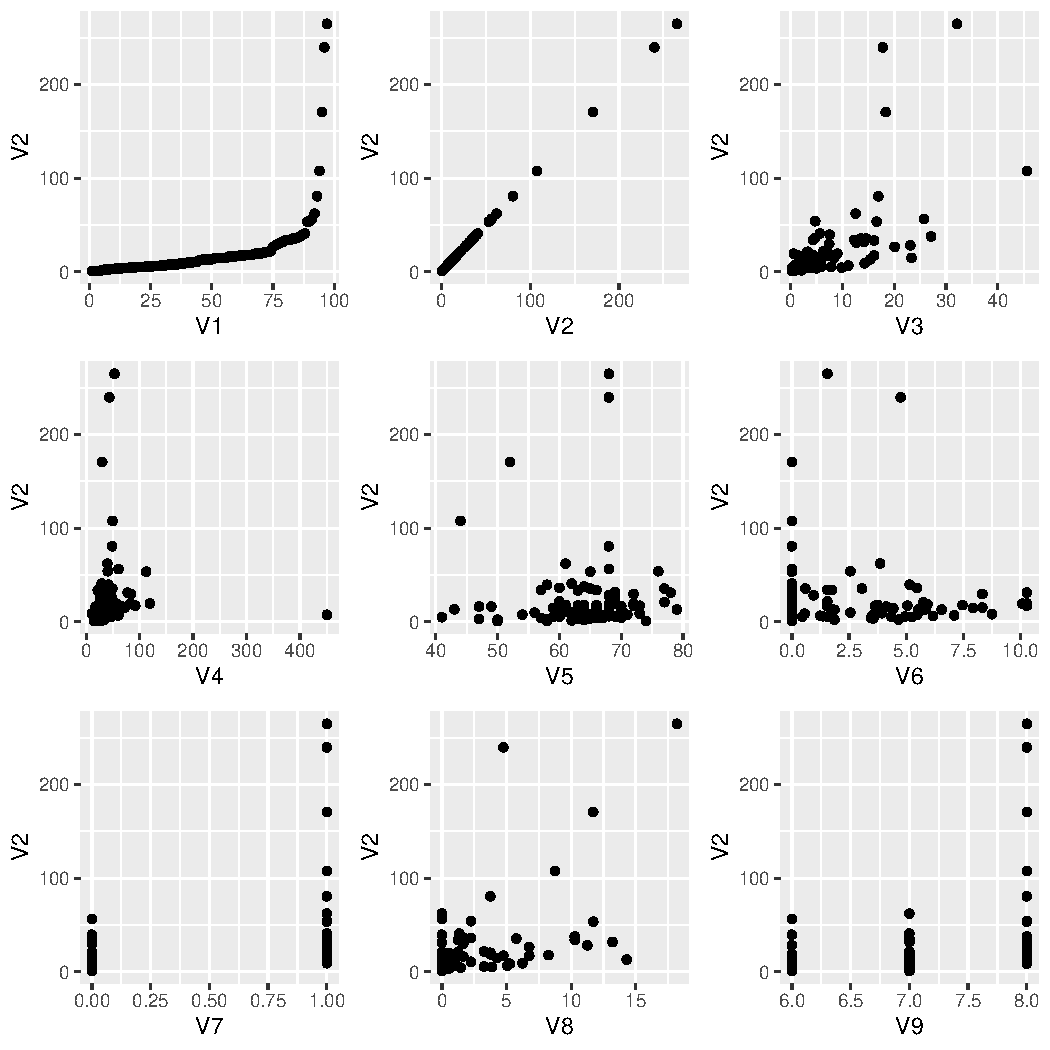
\includegraphics[width=\maxwidth]{figure/unnamed-chunk-4-1} 

\end{knitrout}
\begin{knitrout}
\definecolor{shadecolor}{rgb}{0.969, 0.969, 0.969}\color{fgcolor}
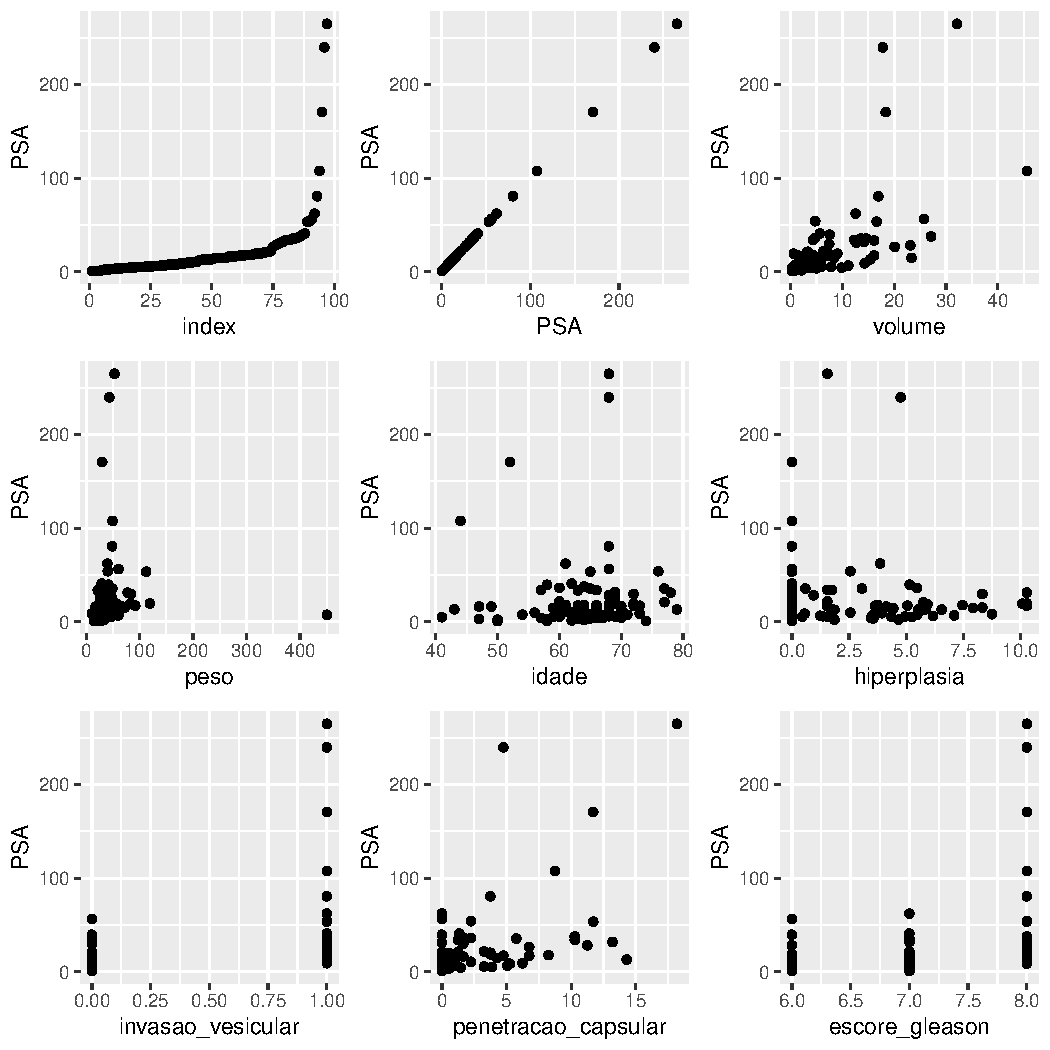
\includegraphics[width=\maxwidth]{figure/unnamed-chunk-5-1} 

\end{knitrout}

%
\section{Inferência e Modelagem}%
\begin{knitrout}
\definecolor{shadecolor}{rgb}{0.969, 0.969, 0.969}\color{fgcolor}\begin{table}[H]
\centering
\begin{tabular}{l|r|r|r|r|r}
\hline
  & Df & Sum Sq & Mean Sq & F value & Pr(>F)\\
\hline
V1 & 1 & 57997.187058 & 57997.187058 & 63.6652953 & 0.0000000\\
\hline
V3 & 1 & 16228.755327 & 16228.755327 & 17.8148037 & 0.0000591\\
\hline
V4 & 1 & 40.078393 & 40.078393 & 0.0439953 & 0.8343472\\
\hline
V5 & 1 & 732.382105 & 732.382105 & 0.8039584 & 0.3723589\\
\hline
V6 & 1 & 1.865549 & 1.865549 & 0.0020479 & 0.9640079\\
\hline
V7 & 1 & 2615.345524 & 2615.345524 & 2.8709452 & 0.0937283\\
\hline
V8 & 1 & 1596.398534 & 1596.398534 & 1.7524158 & 0.1890019\\
\hline
V9 & 1 & 294.318419 & 294.318419 & 0.3230824 & 0.5712088\\
\hline
Residuals & 88 & 80165.377963 & 910.970204 & NA & NA\\
\hline
\end{tabular}
\end{table}


\end{knitrout}

\subsection{Selecção de Variáveis}
\section{Diagnóstico }
\section{Conclusões}

\begin{thebibliography}{9}
\newpage
\bibitem{lamport94}
  Leslie Lamport,
  \textit{\LaTeX: a document preparation system},
  Addison Wesley, Massachusetts,
  2nd edition,
  1994.

\end{thebibliography}
\newpage
\end{document}
